\chapter{Outlet Boundary Condition for Arterial Flow Simulations}

\modinfo{Module name}{\Idx{ArteryOutlet}}
\modinfo{Module subroutines}{\Idx{OutletCompute}, OutletInit, OutletPres, OutletdX, OutletdY}
\modinfo{Module authors}{Esko J�rvinen, Mikko Lyly, Peter R�back}
\modinfo{Document authors}{Esko J�rvinen}
\modinfo{Document created}{April 28th 2006}
\modinfo{Document edited}{April 28th 2006}

\section{Introduction}

Arterial elasticity is a fundamental
determinant of blood flow dynamics in arteries, such as the 
aorta and its daughter vessel, that face the largest displacements and which 
takes care of the cushioning of the stroke volume.  Simulation of such a 
phenomenon requires simultaneous solving of the equations governing both the 
fluid flow and wall elasticity.  To be able to perform accurate 
fluid-strucrure interaction (FSI) simulations, only a segment of the 
circulatory system can be studied at a time. For these 
artificially truncated segments, which are naturally unbounded domains and 
in interaction with the rest of the circulation domain, one should construct
in the numerical models boundary conditions which do not exhibit any
unphysical behaviour, which operates 
transparently, and are also capable to transport a sufficient amount of 
information over the boundary.  

A natural boundary condition at the outlet of a numerical FSI flow model of an 
artery is not a proper choice because it  does not exhibit enough correct 
physiological behavior of the flow, 
and from the point of view of numerical approximation, 
it causes non-physiological reflections of the wave at the boundary. 
If measured data of both the pressure (or velocity) and the wall 
displacement at the outlet boundary are not available, 
%i.e.~the displacement of the wall can not be predescribed, 
the only way to get the outlet boundary of a higher order, 2D or 3D model 
sufficiently specified is to combine the model
with some lower order model, such as a 1D or lumped model.

In order to get the outlet of the arterial FSI model to behave
transparently in such cases when only forward travelling 
waves are considered, a simple characteristic equation of the
of the one dimensional FSI model can be combined
with the higher order model.

\section{Theory}

The conservation equations for a flow in an elastic artery in one 
dimension may be expressed as

\begin{equation}
\left\{ \begin{array}{ll}
{{\partial A}\over{\partial t}} + {{\partial Q}\over{\partial x}} = 0 & \\
& \\
{{\partial Q}\over{\partial t}} + {{\partial}\over{\partial x}}
({{Q^2} \over {A}}) 
+ {{A} \over {\rho}}{{\partial p}\over{\partial x}}= 0, & \\
%& \\
%p = \beta(\sqrt{A}-\sqrt{A_0}),
        \end{array}
\right. 
\label{eq:1Dyhtalot}
\end{equation}

where $Q$ is the volume flow, $A$ the cross section area of the artery, $p$ is 
the pressure and $x$ is the axial coordinate~\cite{hughes2}.  In order to get the 
system (\ref{eq:1Dyhtalot}) close, an equation relating the area 
$A$ to the pressure $p=p(A)$ is derived applying the theory of thin shell 
structures. Assuming a cylindrical shell, and neglecting the rotation on the 
shell cut plane, and the movements of the structure in the axial 
and circumferential directions, as well as applying the Kirchhoff-Love
assumption, the energy balance equations is reduced to

\begin{equation}
{{E~h^3}\over{12(1-\nu^2)}}~{d_R}^{(4)} + 
{{E~h}\over{(1-\nu^2)}}~{{1}\over{{R_m}^2}}~d_R = p, 
\label{eq:enebala}
\end{equation}

where $R_m$ is the radius to the midplane of the wall, $E$, $\nu$ and $d_R$
are the Youngs modulus, the Poisson ratio and the radial displacement of wall,
respectively.  Assuming that the first term on the left side in the
equation (\ref{eq:enebala}) is much smaller than the second term, we 
can give the pressure-area relation in the form

%\[
\begin{equation} 
p = p_{ext}+\beta(\sqrt{A}-\sqrt{A_0}),
\hspace{10mm} \beta={{\sqrt{\pi}hE}\over{(1 - \nu^2 ) A_0}}.
\label{eq:painebeta}
\end{equation} 
%\]

The pressure is scaled to be equal to external pressure $p_{ext}$ 
with corresponding reference artery cross sections area $A_0$.  
%Hereafter we set $p_{ext}$ equal to zero.

The equations (\ref{eq:1Dyhtalot}) and (\ref{eq:painebeta}) form a closed 
system for the simulations of flow in an elastic tubes.  The equations may be 
written in conservative form which is strictly hyperbolic with two distinct 
real eigenvalues 
$\lambda_{1,2} = \bar{u}\pm c$, where 
$\bar{u}={{Q}/{A}}$ is the average axial velocity, 
$c = \sqrt{({{{A}/{\rho_{f}}}) ({{\partial p}/{\partial A}}})} =  
\sqrt {{\beta \sqrt{A} /(2{\rho_{f}})}} $ is the speed 
of sound, and $\rho_{f}$ is the density of blood. The system %of equations 
%(\ref{eq:konservatiivinen2}) 
can be further decomposed into a set of the equations 
for the characteristic variables $W_i$, which are the components of the vector
$W=T^{-1}U ~({{\partial W}\over{\partial U}}=T^{-1}$)
, $U = [A,Q]^{T} ~\cite{godlewski_raviart}$.  These equations are 

\begin{equation}
{{\partial W_i}\over {\partial t}}+
\lambda_i{{\partial W_i}\over {\partial x}}=0,
\label{eq:W-yhtalot}
\end{equation}

and the characteristic variables are 

\[
%\begin{eqnarray}
W_{1,2}= 
%\bar{u}\pm 4c = 
%\bar{u} \pm 2 \sqrt{ {{2}\over{\rho}} } \sqrt{p + \beta \sqrt{A_0}} =
{{Q}\over{A}}\pm 2\sqrt{{{2}\over{\rho_{f}}} + \beta \sqrt{A}}.
\label{eq:Weet}
%\end{eqnarray}
\]

When considering a pulse propagation in a straight, infinitely long homogeneous
conduit, without any bifurcations or other objects which might cause reflections 
of the pulse, i.e.~any backward travelling waves does not exists, the 
computations can be done using only the first of equations in 
(\ref{eq:W-yhtalot}), i.e.

\[
%\begin{equation}
{{\partial W_1(U)}\over {\partial t}}+
\lambda_1(U){{\partial W_1(U)}\over {\partial x}}=0.
\label{eq:ekaW-yhtalo}
%\end{equation}
\]
 
This equation is solved in this Elmer outlet bondary condition for 
arterial flow simulations solver.
The connection of the one dimensional model to the test models at the 
their outlets is done applying the following coupling~\cite{formaggia1}

\begin{eqnarray*}
\left\{ \begin{array}{ll}
dR^{-}=dR^{+}& \\
\sigma^{-}=p^{+}& \\
W_1 = g_1(A^{-},Q^{-},p^{-}),&
        \end{array}
\right. 
\label{eq:jatkuvuusehdot}
\end{eqnarray*}

where $dR$ and $\sigma$ are radial displacement of the artery wall
and fluid traction, respectively.
The superscript '--' denotes the values in the higher order 
models, and superscript '+' to the values in the 1D model. 




%\hspace{10mm} \beta={{\sqrt{\pi}hE}\over{(1 - \nu^2 ) A_0}}.

\section{Keywords} 

\subsection*{Keywords of FlowSolve}

\sifbegin
\sifitem{Initial Condition}{ic id}
For making the initial guess for the characteristic variable $W_1$
\sifbegin
\sifitem{Wnodal} {Variable Coordinate \\ 
Real Procedure "ArteryOutlet" "OutletInit"}
\sifend
\sifend

\sifbegin
\sifitem{Material}{mat id}
Material properties for the one dimensional section.
\sifbegin
\sifitem{Density}{Real}
Density of blood
\sifitem{Artery Wall Youngs Modulus}{Real}
Young's modulus of the artery
\sifitem{Artery Radius}{Real} 
Radius of the artery to the midplane of the artery wall
\sifitem{Artery Wall Thickness}{Real}
Wall thichness of the artery
\sifitem{Artery Poisson Ratio}{Real}
Poisson ration of the artery
\sifend
\sifend

\sifbegin
\sifitem{Solver}{solver id}
Keywords for the one dimensional solver.
Note that all the keywords related to linear solver (starting
with {\tt Linear System})
may be used in this solver as well.  They are defined elsewhere. 
\sifbegin
\sifitem{Equation}{String [Artery Outlet Solver]}
%\sifitem{Time Derivative Order}{[1]}
%\sifitem{Stabilize}{Logical [False]}
\sifitem{Variable}{[Wnodal]}
The variable which is solved 
\sifitem{Variable DOFs}{[1]}
\sifitem{Procedure}{File "ArteryOutlet" "OutletCompute"}{}
The name of the file and the subroutine
\sifend
\sifend

\sifbegin
\sifitem{Equation}{eq id}
The equation section is used to define a set of equations for a body
or set of bodies 
\sifbegin
\sifitem{Artery Outlet Solver}{Logical [True]}
If set {\tt True}, the solver is used.  The name of the solver must
match with the name in the {\tt Solver} section
\sifend
\sifend

\sifbegin
\sifitem{Boundary Condition}{boundary id}
The pressure of the given coordinate direction \texttt{i} at the artery outlet of the
higher order model is set to correspond the value given by the
1D model.  
\sifbegin
\sifitem{Pressure i}{Variable Time \\
 Real Procedure "ArteryOutlet" "OutletPres"}
\sifend
\sifend

\sifbegin
\sifitem{Boundary Condition}{boundary id}
The diameter of the artery in the appropriate direction at the outlet of the
higher order model is set to correspond the value given by the
outlet boundary codition solver.  The subroutines {\tt OutletdX} 
and {\tt OutletdY} are located in the module {\tt ArteryOutlet}
\sifbegin
\sifitem{Displacement i}{Variable Time \\
      Real Procedure "./ArteryOutlet" "OutletdX"}
\sifend
\sifend

\sifbegin
\sifitem{Boundary Condition}{boundary id}
This is the inlet boundary of the one dimensional section which is coupled
with both, the fluid and the solid outlet boundary of the higher order model
\sifbegin
\sifitemnt{Fluid Coupling With Boundary}{Integer} 
\sifitem{Structure Coupling With Boundary}{Integer}
\sifend
\sifend

%\section{Limitations}

%The model can be applied with outlets which surface normals are
%pointing to the positive z-coordinate direction.

\begin{figure}[tbhp]
\begin{center}
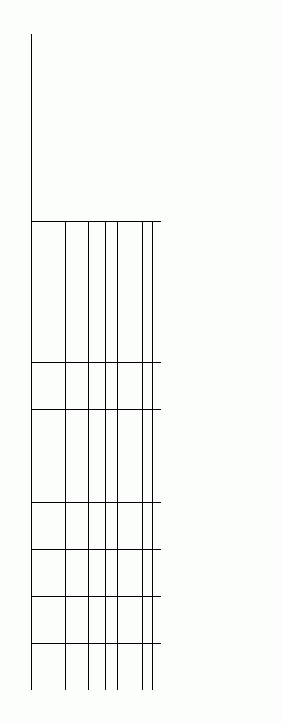
\includegraphics[width=0.16\textwidth]{grid.png}
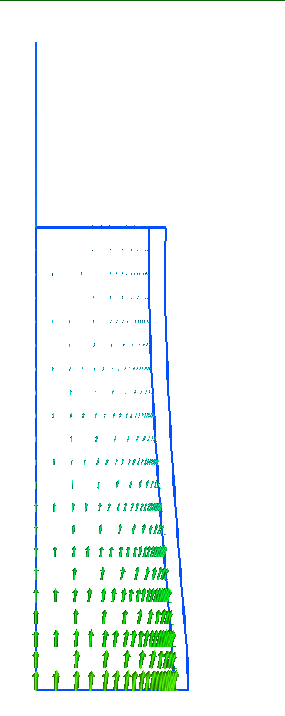
\includegraphics[width=0.16\textwidth]{t10.png}
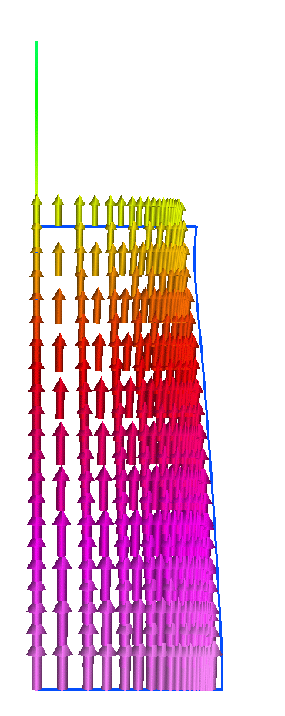
\includegraphics[width=0.16\textwidth]{t20.png}
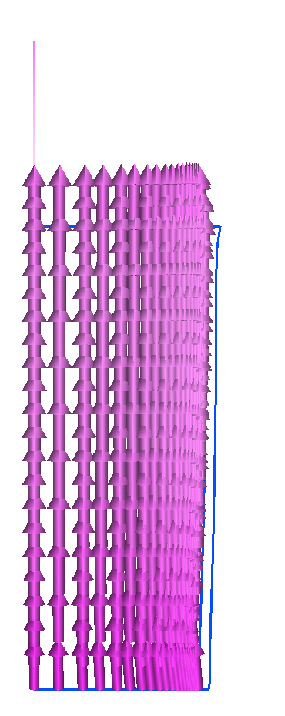
\includegraphics[width=0.16\textwidth]{t30.png}
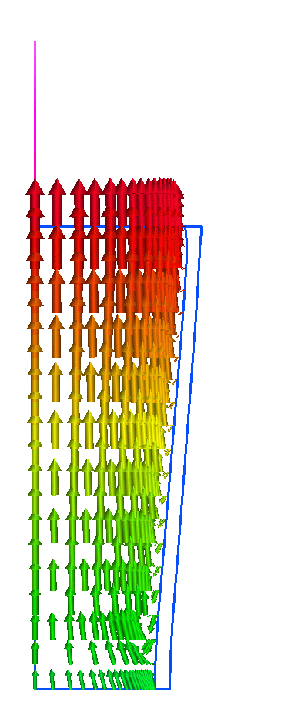
\includegraphics[width=0.16\textwidth]{t40.png}
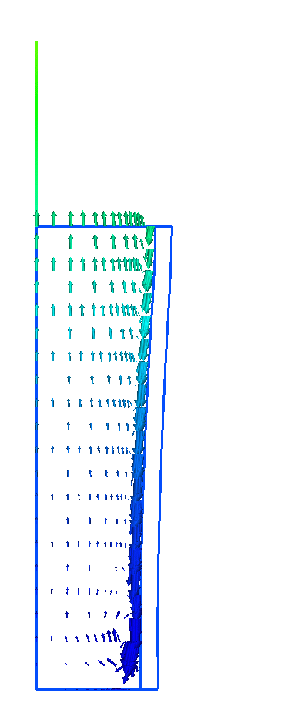
\includegraphics[width=0.16\textwidth]{t50.png}
\end{center}
\caption{An example of the model results: pressure pulse prapagation in a 2D axisymmetric 
model combined with an 1D model.}
\end{figure}

\bibliography{elmerbib}
\bibliographystyle{plain}


